\chapter{Applying the PSO to the FAP}
\label{chpt:psoapplicationFAP}
\section{Introduction}
PSO, as discussed previously (see page \pageref{sec:PSO}), is an algorithm that is largely based on the flying behaviour exhibited by a flock of birds. This is why the core of the algorithm is based upon vector mathematics, with new positions and velocities being calculated after each iteration of the algorithm. Thus a D-dimensional vector represents each particle position and is then simulated by flying through the D-dimensional space using the velocity equation (see section~\ref{sec:particleVelocity} on page~\pageref{eq:velocityupdate}).

Most of the problems to which PSO has been applied to date have been problems where the position of particles has a constant D-dimensional space. In formal terms, therefore, \emph{the dimensionality of a particle position in its entirety is constant}. Therefore, each particle has a position which is defined in a set dimension like 2D where a position is represented at $x$ and $y$ coordinate pairs.

This constant dimensionality introduces an intriguing problem if one wants to apply the PSO to an inherent multidimension problem like the FAP. This chapter deals with how the PSO was applied to the FAP.

Firstly, the particle position is represented in the frequency planning domain is defined. This definition of the particle position is important because it plays a central part in
the movement of particles through the Frequency planning domain. A description is then given of how each position is evaluated as well as the fitness function that the PSO will use in the FAP domain.

Arguably the most important part of the swarm is how the velocity of a particle is calculated and then moving it to a new position in the problem space. The velocity update is important, as it is the primary means by which the algorithm searches problem space.

As was discussed in section~\ref{sec:psoonfap}, applying the PSO to the FAP introduces a variety of challenges. One of the challenges is how exactly one ``flies'' a frequency plan towards another frequency plan. This is an important question that needs to be addressed as the PSO algorithms have no other way of searching the problem space by any other means.

To be able to allow the PSO to operate in the FAP space custom velocity functions had to be developed to enable the particles of the swarm to move. These velocity functions that were developed will expanded on in section~\ref{sec:velocityFAP}. 

Developing custom velocity functions for the PSO was simply not enough to achieve good results with the PSO. Therefore more innovations needed to be made to improve the solution quality of the PSO. In section~\ref{sec:buildglobalbest} a new mechanism is presented for selecting the global best which enabled the PSO to get better fitness values and therefore direct the swarm more towards better solutions. 

Finally, the chapter will conclude with how the swarm utilises history to produce better results to enable the PSO to further improve the solution quality.
\section{Position in the Frequency Planning Domain}
In this section a description is given of what a position is in the frequency planning domain. First a frequency plan is defined and the general structure to represent such a plan is provided. The section will conclude with the hard and soft constraints and how the constraints aid in creating a frequency plan that is suitable for a network.

A frequency plan, is almost exactly what the name implies: A plan that outlines frequency usage for a mobile telecommunication network. The benchmark problems that were used to test the developed PSO all pertained to cellular phone networks and were presented in section~\ref{sec:FAPBenchmarks}. For cellular networks, the frequency plan outlines which frequency must be allocated to which transceiver.

With this basic definition, the problem is deceptive as one naturally assumes that there are an infinite number of frequencies that can be used or the number of frequencies available for assignment is more than the number of transceivers in the network. 

The reality is that there are only a finite number of frequencies available for cellphone transmissions, as was discussed in chapters~\ref{chpt:celltech} and \ref{chpt:fap}. Hence a regulatory body needs to assign wireless spectrum to cellphone network operators for use in their networks. A regulatory body is needed because, if a network operator uses just any frequency it wants, it is bound to interfere with someone else also utilising the same frequency.

A network is not assigned to the entire wireless spectrum for wireless communication, but rather only a subset is assigned to the network. If one observes the FAP benchmark problems the PSO was applied to (see section~\ref{sec:FAPBenchmarks}) for instance Siemens1, the allotted spectrum is from frequency 16 to 90. Which gives the network operator 74 frequencies to use in its network without considering other constraints. 

Besides the electromagnetic constraints that are also applicable here, there are regulatory constraints, for instance frequencies in the spectrum that are by no means allowed to be used. These frequencies are referred to as globally blocked frequencies and are hard constraints. An in-depth discussion of these constraints was given in section~\ref{sec:Interference}.

As discussed in chapters~\ref{chpt:celltech} and \ref{chpt:fap}, a cellphone network is divided into a number of cells, and each cell requires a certain number of transceivers to service its corresponding area. 

The number of transceivers is based on the expected volume of traffic that a particular cell will experience at peak network usage. Some cells might be located in highly populous areas, which means the potential traffic that cell might need to handle during peak network usage is very high and thus the cell has more than one transceiver to handle the potential traffic. With cells that are located in areas that have a low population, the potential traffic the cell might experience during peak network usage is low and thus the cell only has one transceiver to handle potential traffic.

Based on the amount of traffic a cell needs to handle, the number of transceivers differs; thus in a frequency plan not all cells have the same number of transceivers, otherwise a frequency plan can be modelled as a series of constant D-dimensional vectors, where the D represents the number of transceivers. 
~
\begin{figure}[ht]
	\centering
	\setlength \fboxsep{0pt}
	\setlength \fboxrule{0.5pt}
	\fbox{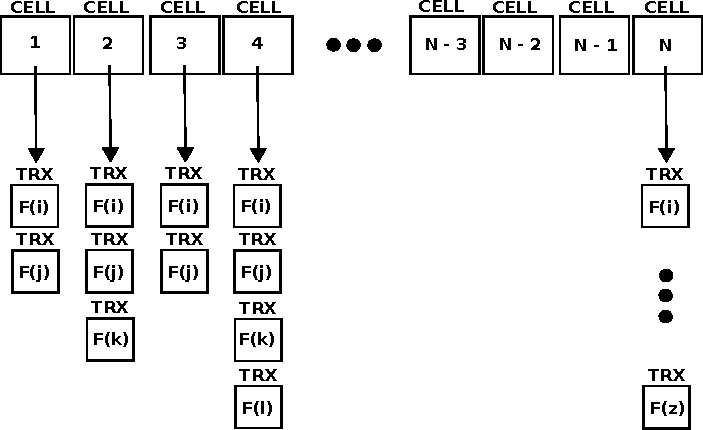
\includegraphics[width=4.8in, height=3.5in]{./pictures/fapPlanDiagram.pdf}}
	\caption{The structure of a frequency plan}
	\label{fig:fapPlan}
\end{figure}
~
As can be seen in figure \ref{fig:fapPlan} a cellular network can have any number ($N$ in the figure) of cells to attain the desired coverage over the geographical landscape. In the COST 259 benchmark problems the cellular networks have a large number of cells that range from 500 to more than 1 000. 

The most important part of the plan is the actual transceivers within each cell. In figure~\ref{fig:fapPlan} it can be clearly seen how the number of transceivers (TRXs) varies from one cell to the next. $F(i)$ is a frequency at position $i$ from the available usable spectrum. 

Based on the structure of the plan depicted in figure \ref{fig:fapPlan} there is no concept of which cell interferes with which other cell and if there is indeed interference, the extent of this interference. Not all this information is part of the plan. Instead this information, for the purpose of this research is supplied by the COST 259 benchmark. 

The interference information is referred to as the interference matrix. A definition of the structure of an interference matrix was given in section~\ref{sec:Interference}. As discussed, each entry references two cells' entries: Cell A and Cell B. Along with the entry the amount of interference that occurs when Cell B interferes with Cell A is also listed\footnote{Interference occurs based on the electromagnetic constraints as defined in chapter~\ref{chpt:fap}}.

A frequency plan is a possible solution to the FAP. Therefore in the PSO that was developed each particle's position in the solution space is represented by a frequency plan. As illustrated in figure~\ref{fig:fapPlan}, a frequency plan is just a series of cells, where each cell has a set of transceivers; thus in the PSO algorithm a plan is actually represented as an array of cells. This enables the algorithm to access particular cells in a plan by index as can be observed in listed algorithms~\ref{alg:velocitymethod1} and ~\ref{alg:velocitymethod2}. 

Before the particles can actually start to move around in the FAP space, they first need to be assigned positions. In the developed PSO listed in algorithm~\ref{alg:FAPPSO} line 1 the first operation that the algorithm executes is to initialise all the particles in the swarm. A particle position in the algorithm is initialised by assigning it a random position; thus a frequency plan (representing a position) is randomly generated by the algorithm.
\begin{algorithm}[H]
\label{alg:FAPPSO}
\caption{The FAP PSO Algorithm}
\begin{algorithmic}
\State $s_n$ = Initialize Swarm $s_n$
\While{Termination criterion not met}
	\State EvaluateSwarm($s_n$)
	\State UpdateGlobalBest($s_n$)
	\State UpdateSwarmMovement($s_n$,$gbest$)
\EndWhile
\end{algorithmic}
\end{algorithm}


The position is purely random in that the only considerations made by the position generator are that valid frequencies are assigned to transceivers installed at cells. Thus the generator does not check whether a frequency has already been assigned in the current cell or any other considerations. The intended purpose of the generator is just to place a particle in the problem space, not the premature start of the optimisation process.

Since particles are able to occupy positions in the FAP space the PSO algorithm is now able to move them around in the problem space. As mentioned previously, moving particles through the frequency plan solution space introduces an interesting problem due to the multidimensionality of a plan. A discussion of how particles are moved from one position to another through the solution space is provided in section \ref{sec:velocityFAP}

In the next section an explanation is given on the fitness function that determines the desirability of a particular particle's position or rather the frequency plan its position represents.
\section{The Fitness Function}
The fitness function rates the desirability of a particular particle's position in the problem space.

As discussed in the previous section, the COST 259 benchmark problems provide an interference matrix that lists the total amount of interference that occurs when a pair of cells interfere. As outlined in the structure definition (see section~\ref{sec:Interference}) each entry in the interference matrix defines a pair of cells that are said to interfere, along with two additional values. The first value is referred to as co-channel interference and is the total amount of interference that will occur on the communication link when the allocated frequency of one transceiver is equal to a transceiver in the other cell that is listed in the interference matrix. 

The second value is called adjacent channel interference and it is the total amount of interference that will occur on the communication link when the allocated frequency of a transceiver in one cell differs by 1 from another frequency allocated to the transceiver from the other cell that is listed in the interference matrix.

Particles move towards other particles because the other particles have indicated (through information sharing) that the positions they occupy are very lucrative and thus they have found potentially good solutions. The only way particles can know the lucrativeness of the position they occupy is if the position is evaluated with a fitness function. Thus the lucrativeness of a position is actually the fitness value obtained from the fitness function. 

Since a particle position is defined as a frequency plan, a procedure is needed that calculates the fitness of a frequency plan. With the FS-FAP the primary concern is to keep interference to a minimum. Therefore in the PSO that was developed the fitness value is the total amount of interference generated by all the cells with their allocated frequencies. 

The evaluation procedure goes through each pair of cells defined in the interference matrix where it looks up both cells in the frequency plan. The second cell is said to interfere with the first cell. Therefore each transceiver in the first cell is checked against all the transceivers of the other cell. Depending on whether the frequencies differ from each other, the fitness procedure adds either co-channel or the adjacent channel interference to a summing variable. This procedure is mathematically defined in chapter 3 (see page \pageref{E:costFunction} for the formal equation) and algorithm~\ref{alg:fapcost} is the pseudocode of the implement equation used by the PSO. 

\begin{algorithm}
\caption{FAP Cost Function}
\label{alg:fapcost}
	\begin{algorithmic}[1]
	\Require normalCell
	\Require interferingCe;;
	\State $totalInterference \leftarrow $0
	\For{Each TRX $trx_i$ in interferingCell}
		\For{Each TRX $trx_j$ in normalCell}
			\State $interference \leftarrow 0$
			\State $difference \leftarrow$ $|trx_i - trx_j|$
			\If{difference is 0}
				\If{coChannelInterference $\leq$ minInterferenceThershold}
					\State $interference \leftarrow interference + 0$
				\Else
					\State $interference \leftarrow interference + coChannelInterference$
				\EndIf
			\Else
				\If{difference is 1}
					\If{adjChannelInterference $\leq$ minInterferenceThershold}
						\State $interference \leftarrow interference + 0$
					\Else
						\State $interference \leftarrow interference + adjChannelInterference$
					\EndIf
				\EndIf
			\EndIf
			\State $totalInterference \leftarrow totalInterference + interference$
		\EndFor
	\EndFor
	\end{algorithmic}
\end{algorithm}

As can be seen in algorithm~\ref{alg:fapcost} not all interference values are added to the total amount of interference variable. The COST 259 benchmarks define a minimum tolerable interference variable. This means that if a given interference value is either equal to or less than this defined value the interference generated is negligible and can be disregarded as it will not have a noticeable impact on the communication link.

In the next section a description is given of how particles are moved from one iteration to the next using frequency plans as positions in the solution space.
\section{Velocity Function for Frequency Planning}
\label{sec:velocityFAP}
The elocity function is arguably the core of the PSO algorithm. It is the procedure by which particles in the swarm move from one point to another in the solution space. 

The velocity function does not blindly move a particle from one point to another, but instead it takes the particle history into account as well as the best particle in the swarm. Therefore the velocity function is the core means by which the swarm explores the solution space. A more thorough explanation is provided in section~\ref{sec:particleVelocity}.

The development of a velocity function that is suitable for particles to move from one frequency plan to another is covered next. The section will start off with the first velocity function that was developed. With each method discussed, the problems associated with it will also be mentioned. 

This section will conclude with the second method that was developed and that is also the primary method the developed PSO uses.

\subsection{Movement in the Frequency Planning Domain}
The standard velocity equation works on the basis of vector mathematics. Each particle has a velocity and position, which is represented by a standard mathematical vector. The standard equation alters the direction of the particle to move to a more promising position in the solution space that is in the general direction of the global best particle and a previous personal best position the particle held..

Vector mathematics has standard basic operations defined for adding, subtracting and multiplying; hence applying the PSO to problems that are either mathematical functions or problems that map well to the vector domain is a defined process. With regard to the frequency planning domain an important question needs to be answered: How can one multidimension frequency plan be moved to another?

With any difficult problem it is better to break the problem down into its most basic constructs and then solve each piece individually until the problem as a collective is solved. This technique is also commonly known as divide and conquer. This technique was first applied to the nature of a frequency plan.

A frequency plan is a plan that consists of a series of different cells that are in use in the network. The plan specifies the frequencies that each individual transceiver installed at a cell must use for communication. Thus a frequency plan can broken up into three important constructs:
\begin{enumerate}
\item A plan is a list of different cells.
\item Each cell in a plan has a list of transceivers that it has installed.
\item Each installed transceiver has a single number allocated to it called the frequency. This frequency is used for communication.
\end{enumerate}

Now that a frequency plan has been broken up into its constructs, the question of how to move one frequency plan to another can be rephrased. How does one move a frequency allocated to a \emph{transceiver} in a particular \emph{cell} of one frequency plan to another frequency of the \emph{same} transceiver and cell in another \emph{different} plan? An important realisation needs to be noted here. In the PSO at any one time the algorithm is only considering two positions and for the FAP the two positions are frequency plans. Both plans are \emph{identical} except for the specific that frequencies transceivers use. Thus a cell that exists in the one plan, also exists in another plan. Both the cells have exactly the same number of transceivers installed; only the frequencies each individual transceiver uses for communication differ.

Using this realisation, the conclusion can be made that the velocity equation can only work with the frequencies assigned to transceivers. Therefore a potential velocity equation mechanism needs to operate on the finest granularity of a frequency plan, i.e. the frequencies.

The principle on which the first velocity method developed is based, is for the movement of the swarm to be at a much finer granularity and hence movement is based on frequencies. Therefore when a particle needs to move towards a global best particle, the velocity procedure goes into the intricate details of the particle wanting to move and the global best particle. The procedure goes into each cell defined in the frequency plan represented by the standard particle as well as the global best particle to be able to access each installed transceiver.

To be able to move from one frequency plan to another by utilising the standard velocity equation, the equation needs to be broken up into its smaller operations. In this way, small operations can be developed that perform the same function as the individual parts. 

The velocity equation in section~\ref{sec:particleVelocity} can be broken up into the following parts:
\label{lst:velocitybreakup}
\begin{itemize}
\item \textbf{Subtraction} --- $pbest - x_i(t)$ --- (SubtractionResultPbest) and $gbest - x_i(t)$ --- (SubtractionResultGbest)
\item \textbf{Multiplication} --- $c_1\phi_1 * SubtractionResultPbest$ --- (MultiPbestResult) and $c_2\phi_2 * SubtractionResultGbest$ --- (MultiGBestResult)
\item \textbf{Addition} --- $v_i(t) + MultiPbestResult + MultiGBestResult$
\end{itemize}
There are no mathematical constructs that define how two frequency plans are added together or subtracted, let alone multiplied. As discussed earlier, a frequency plan is just a series of cells that have frequencies and these frequencies are numbers that internally are just integers and there are mathematical constructs that define how two integers should be added, subtracted or multiplied. Both velocity methods that were developed utilise the basic principle that on a fine granularity of a frequency plan one is merely working with integers.


The first velocity method is listed in algorithm~\ref{alg:velocitymethod1}. Velocity method 1 works on the principle of moving one cell in a particular frequency plan to the same cell in a different frequency plan. As noted earlier, the cells are the \emph{same}, but the frequencies that have been allocated to each transceiver within a cell differs. Thus in velocity method 1, each cell has an array of transceivers. The array of transceivers contains the individual frequency numbers that have been allocated to a cell.
\begin{algorithm}[H]
\caption{Velocity Method 1}
\label{alg:velocitymethod1}
	\begin{algorithmic}[1]
	\Require currentParticle
	\Require globalBestParticle
	\State $pbest \leftarrow $currentParticle position
	\State $gbest \leftarrow $globalBestParticle position
	\State $localCoeff \leftarrow getLocalCoefficient()$
	\State $globalCoeff \leftarrow getGlobalCoefficient()$
	\State $pBestSubtractResult \leftarrow $Subtract current Particle position from pbest
	\State $gBestSubtractResult \leftarrow $Subtract current Particle position from gbest
	\State $a \leftarrow $Multiply localCoeff with pBestSubtractResult and a random value
	\State $b \leftarrow $Multiply globalCoeff with gBestSubtractResult and a random value
	\If{first time velocity is calculated for current Particle}
		\State $currentParticle.Velocity \leftarrow $Add a and b
	\Else
		\State $abAdditionResult \leftarrow $Add a and b
		\State $inertia \leftarrow getInertia()$
		\State $newVelocity \leftarrow $Add abAdditionResult and currentParticle.Velocity
		\State $currentParticle.Velocity \leftarrow $Multiply inertia with newVelocity
	\EndIf
	\State $currentParticle.Position \leftarrow $Add currentParticle.Velocity and currentParticle.Position
	\State SanatizePosition(currentParticle.Position)
	\end{algorithmic}
\end{algorithm}

Velocity method 1 actually moves one array of transceivers to another array of transceivers. This is why, if one observes lines 5 -- 17 in algorithm~\ref{alg:velocitymethod1}, each particle position is passed to methods that are named Subtraction, Multiplication and Addition. As discussed in the previous section, each position of a particle is actually a frequency plan.


The first method that is used to calculate the velocity of a frequency plan, is the first basic operation defined in the velocity equation, namely subtraction, as can be observed from algorithm~\ref{alg:arraySubtract}. The particular algorithm expects two positions to be given to it: the position it must be moved from and the position it must be move to. Because each position is a frequency plan that contains an array of cells, a for-loop is started on line 1 that allows the algorithm to go through each cell that is defined in the frequency plan. Each cell has a number of transceivers, each with an assigned frequency. 
\begin{algorithm}[H]
\caption{Subtract One Position From Another} (Method 1)
\label{alg:arraySubtract}
\begin{algorithmic}[1]
	\Require fromPosition
	\Require toPosition
	\For{Each cell $c$ in fromPosition}
		\For{Each transceiver $f_{trx}$ in $c$}
			\State $t_{trx} \leftarrow$ Get same $f_{trx}$ in toPosition
			\State $f_{trx} \leftarrow f_{trx} - t_{trx}$
		\EndFor
	\EndFor
\end{algorithmic}
\end{algorithm}


To be able to subtract two transceivers from each other, the algorithm needs access to a particular transceiver of a cell. The algorithm gains this access by entering another for-loop based on the number of transceivers a cell has, as can be observed to occur in line 2. Within this for-loop the actual subtraction of transceivers occurs.

The algorithm first obtains the exact same transceiver in the toPosition frequency plan. This operation is quick, as the two plans are identical except for the frequencies assigned to transceivers for each cell. Thus the algorithm is able to refer to the cell and specific transceiver in the toPosition plan by the same index it utilises to access the cell and transceiver in the fromPosition.

Once the toPosition plan transceiver frequency value has been obtained, the algorithm performs a standard integer subtraction as seen in line 4 of algorithm~\ref{alg:arraySubtract}.
After the subtraction algorithm is completed, a position is returned which is the result of subtracting the fromPosition from the toPosition. Using this result the velocity method 1 algorithm is now ready to apply the next operation in the velocity update equation, namely multiplication which is depicted in algorithm~\ref{alg:arrayMultiply}.

\begin{algorithm}[H]
\caption{Multiply Position by a Value (Method 1)}
\label{alg:arrayMultiply}
\begin{algorithmic}[1]
	\Require fromPosition
	\Require value
	\Require mustRandom
	\For{Each cell $c$ in fromPosition}
		\For{Each transceiver $trx$ in $c$}
			\If{must multiply with random number}
				\State $trx \leftarrow trx * value * random()$
			\Else
				\State $trx \leftarrow trx * value$
			\EndIf
		\EndFor
	\EndFor
\end{algorithmic}
\end{algorithm}

The multiplication algorithm is where the local Coefficient and the global coefficient\footnote{Local coefficient is the cognitive component and the global coefficient is the social component. These components are discussed in section~\ref{sec:psointro}} defined for the PSO are multiplied into a position, i.e. frequency plan. As with the subtraction algorithm the multiplication algorithm enters two for-loops. The first for-loop is to access each cell defined in the frequency plan. The second loop allows the algorithm to access each transceiver within a particular cell. These for-loops can be observed to occur in algorithm~\ref{alg:arrayMultiply} in lines 1 and 2.

Once the algorithm is able to access each individual transceiver and get its assigned frequency, it is able to perform the multiplication operation. As can be observed in the algorithm in line 3 the algorithm checks whether it needs to multiply the frequency by an additional random number besides the $value$ passed to the algorithm. The reason this is done is that multiplication is required in the PSO in the following cases:

\begin{itemize}
\item The inertia case --- $0.5 * v(t+1)$, where 0.5 is the inertia value and $v(t+1)$ is velocity that has already been calculated for a particular particle $t$. Note, a velocity that has been calculated is still a frequency plan.
\item Standard velocity calculation randomisation case --- As can be observed from the velocity equation~\ref{eq:velocityupdate} and also from the multiplication bullet point on page~\pageref{lst:velocitybreakup}, the equation requires that a position be multiplied by a coefficient $c_1$ or $c_2$ and then a random value $\phi_1$ or $\phi_2$. 
\end{itemize}

Regardless of which case is executed, the actual operation that is performed is integer multiplication, which therefore means that even though the inertia and random numbers are decimal, the fractional component of the result is discarded. Channels are integers so the loss of the fractional component is warranted as it is of no use.

As per the last bullet point on page~\pageref{lst:velocitybreakup} the last basic operation that occurs in the velocity equation is an integer addition operation. Algorithm~\ref{alg:arrayAdd} is the addition procedure used by velocity method 1 (algorithm~\ref{alg:velocitymethod1}).
\begin{algorithm}[H]
\caption{Add One Position to Another (Method 1)}
\label{alg:arrayAdd}
\begin{algorithmic}[1]
	\Require fromPosition
	\Require toPosition
	\For{Each cell $c$ in fromPosition}
		\For{Each transceiver $f_{trx}$ in $c$}
			\State $t_{trx} \leftarrow$ Get same $f_{trx}$ in toPosition
			\State $f_{trx} \leftarrow f_{trx} + t_{trx}$
			\State Bound($t_{trx}$)
		\EndFor
	\EndFor
\end{algorithmic}
\end{algorithm}

In the addition algorithm, as with multiplication and subtraction, two for-loops are started as can be observed in lines 1 -- 2. The algorithm first starts iterating through all the cell's present in the fromPosition frequency plan and then within the cell for-loop starts another for-loop which iterates through each cells transceivers. Inside the transceiver for-loop the algorithm actually performs the addition of two frequencies.

Two frequencies are added based on integer addition. Once the fromPosition cell transceiver is accessed, the algorithm retrieves the exact transceiver and cell in the toPosition in order to get its allocated frequency value. After both values have been retrieved the algorithm performs the addition as can be observed in line 4 of algorithm~\ref{alg:arrayAdd}.

The addition operation is the last operation that occurs in the velocity equation and is also the only operation that occurs when the resultant velocity is applied to the current position of a particle as in equation~\ref{eq:positionupdate}. Since the addition operation is also used in the final position update of the particle, its last operation in the transceiver loop a bound operation. 

The purpose of the bound operation is to keep the frequencies within valid value ranges.
\subsection{Keeping Frequencies Bounded}
In the previous section the first velocity method that was developed was discussed. The velocity method is important as it calculates the direction and next position of a particle in the problem space, where the problem space is the FAP and a position of a particle is a possible frequency plan. With the velocity method defined, the swarm is now able to move around in the problem space, but this alone is not enough. The swarm has no concept of the constraints\footnote{Constraints in the FAP are discussed in chapter~\ref{chpt:fap}} that are imposed inherently by the domain as well as the network for which a frequency plan is being created.

Due to the swarm not having a concept of the constraints a constraint handling mechanism needs to be used. Each of the methods discussed in this section fall under the category of using the \emph{repair method} which is discussed in section~\ref{sec:chm}

The first method that was developed was the BoundValue method and is depicted in algorithm~\ref{alg:boundvalue}.
\begin{algorithm}[H]
\caption{BoundValue Method}
\label{alg:boundvalue}
\begin{algorithmic}[1]
	\Require Position
	\For{Each cell $c_i$ in Position}
		\For{Each transceiver $trx_j$ in $c_i$}
			\State $trx_j = \left|trx_j\right|$
			\If{$trx_j \geq maxChannelValue$}
				\State $trx_j = minChannelValue + (\text{$trx_j$ mod $maxChannelValue$})$
			\Else 
				\If{$trx_j \leq minChannelValue$}
					\State BoundValue($trx_j + minChannelValue$)
				\EndIf
			\EndIf
		\EndFor
	\EndFor
\end{algorithmic}
\end{algorithm}
The constraints that are imposed are usually some part of the spectrum that may under no circumstances be used anywhere in the network, which as discussed in chapter~\ref{chpt:fap} is known as globally blocked frequencies. Some frequencies that are only allowed to be used in certain parts of the network are known as locally blocked frequencies. Then of course the swarm also needs to take into account the electromagnetic constraints\footnote{Discussed in section~\ref{sec:Interference}}.

The velocity function used by the PSO needs to be altered to make the swarm in some sense more aware of the domain it is operating in and hence keep the particle positions bounded within the allowable search space. By not bounding particle positions in the FAP problem space, transceivers of some cells might be assigned a frequency that is not allowed or not even allocated to the network. The PSO will accept this assignment since the fitness function operates on the assumption that under no circumstances will these invalid frequencies be assigned and thus does not penalise invalid assignments.

To keep assigned frequency values to transceivers in the allocated spectrum of the network a boundary check needs to be added to the velocity method. The purpose of the boundary check is to validate all assignments in a position, i.e. the frequency plan that a particle currently occupies, and if any assignments violate the defined boundary constraints then it must take the violating value and modify it to be in the acceptable value range.

The boundary check that is used by velocity method 1 operates on the basis that for any range of values there is a defined lower bound (a minimum value) and upper bound (a maximum value). The frequency boundary check is only applied when one of the following conditions is met after the calculated velocity has been applied to the current position:
\begin{itemize}
\item If a frequency allocated to a transceiver is above the maximum allowable frequency (upper bound) given to the network. 
\item If a frequency allocated to a transceiver is below the minimum allowable frequency (lower bound) given to the network.
\end{itemize}

As can be seen in line 5 of algorithm~\ref{alg:boundvalue}, a mod operation is applied to the value to bring it within the allowable range. The integer mod operation is similar to integer division, the only difference being in the result that is produced. Division produces the result of two numbers being divided. Mod produces the remainder of two numbers being divided. If two numbers divide perfectly into one another there will not be any remainder; if the numbers do not divide perfectly into one another there will be a remainder. 
\begin{align}
	10 mod 50 =& 10 \\
	60 mod 50 =& 10 \\
	50 mod 50 =& 0 \\
	100 mod 50 =& 0 \\
	35 mod 50 =& 35 
\end{align}

As can be seen in the above example mod operations, any value that is modded will be kept in the range $[0,50]$. With regard to frequencies, the following occurs: If, for instance, the maximum allowable frequency is 50, and the transceiver has a frequency value (after velocity) of 56, the 56 value is modded by 50 to produce a value of 6. This modded value is then added to the minimum allowable frequency. In essence, the value is wrapped around to always be within acceptable range. 

The difficult case is when the frequency value is lower than the minimum frequency given to the network. This is because modding the frequency value has no effect. For example, if the lowest allowable frequency is 20 and the transceiver value after movement is 15, modding the transceiver value of 15 by 20 has no effect. To solve this, the following options are then considered:

\begin{enumerate}
\item First subtract the lower value from the minimum allowable frequency. Then add the result to the minimum allowable frequency. The resultant value is checked again as to whether it oversteps the bounds of the maximum allowable frequency and is bounded accordingly.
\item Add the lower value to the minimum allowable frequency. The resultant value is checked as towhether it oversteps the bounds of the maximum allowable frequency and is bounded accordingly.
\item Repeatedly subtract the lower value from the maximum allowable frequency until the resultant frequency is within the acceptable frequency range.
\end{enumerate}

An important notion to consider is that, based on the velocity equation, it is entirely within the realm of possibility that a frequency value after movement might contain a negative value. As can be seen in line 3 of algorithm~\ref{alg:boundvalue} the algorithm solves this problem by first taking the absolute value of the negative frequency value. The boundary check then treats the now positive frequency value as a normal value that needs to be bounded.

It is better to use frequency index values rather than actual frequency values for frequency plans, and this is explained below.
\subsection{Using Indices instead of Frequencies}
\label{sec:velocityFAP2}
As discussed in section~\ref{sec:velocityFAP} and as can be observed from algorithm~\ref{alg:velocitymethod1}, the first velocity method that was developed for the PSO worked with raw frequency values. This is not ideal since upon closer inspection the frequency range that the swarm used to move around was indeed incorrect. The bound value algorithm only keeps frequencies within a minimum and maximum allowable frequency range, but globally blocked frequencies and locally blocked frequencies can be in between this minimum and maximum frequency range. 

With velocity method 1 and the PSO using raw frequency values, the swarm increasingly moved towards allocating these blocked frequencies to trans-ceivers since the fitness function does not penalise the use of blocked or invalid frequency values. This is partly due to the fact that these values are under no circumstances allowed to be used and thus the fitness function is not designed to check for these values explicitly to impose a penalty.

Frequency plans that utilise these blocked frequencies are invalid and cannot be used. If a network were to use a plan that uses blocked frequencies, it could cause unexpected interference to other services and the network could be fined by the governing body that controls the spectrum. A bare minimum requirement then is that the PSO must generate valid frequency plans and hence swarm particles can only occupy valid positions. The following options were presented to solve the problem of particles moving towards invalid positions and hence having invalid frequency plans:
\begin{enumerate}
\item Modify the fitness function to penalise a frequency plan if it uses any globally blocked frequencies or locally blocked frequencies.
\item Instead of letting the swarm work with raw frequency values, rather let it work with indices of an array. The array index values indicate positions in an array that has been pre-filled with only \emph{valid} frequencies. Thus the swarm then moves around in a range from 0 to $F$, where $F$ is the size of the frequency array.
\end{enumerate}

With the first solution, the fitness function would have to be modified to impose a penalty if a prohibited frequency value were used. The first proposed solution was disregarded because it introduces complexity which can be completely avoided with the second proposed solution.

With the second solution the fitness function does not have to be modified and the boundary check is simplified since there is no need to check for a lower bound. The boundary check now only has to check for negative index values and whether the upper bound, which is now the size of the array, is violated. 

The second method is also a method known in constraint handling as \emph{preserving feasibility} (see section~\ref{sec:chm} for a discussion on constriant handling methods). By using only valid frequencies the search space is even more constricted to only feasible solutions.


Working with index values rather than with raw frequency values led to  a second velocity method. Algorithm~\ref{alg:velocitymethod2} is the pseudocode for the second velocity method. The second velocity method differs from velocity method 1 due to it being designed to only work with indices of an array.
\begin{algorithm}[H]
\caption{Velocity Method 2}
\label{alg:velocitymethod2}
\begin{algorithmic}[1]
	\Require currentParticle
	\Require globalBestParticle
	\State $currPos \leftarrow$ currentParticle position
	\State $pbestPos \leftarrow$ currentParticle best position
	\State $gbestPos \leftarrow$ global best particle position
	\For{Each cell $c$ in $currPos$}
		\State $c_{pbestPos} \leftarrow $ Same cell in $pbestPos$
		\State $c_{gbestPos} \leftarrow $ Same cell in $gbestPos$
		\State $movedIndices \leftarrow $MoveIndices($c_{pbestPos},c,c_{gbestPos}$)
		\If{First time velocity is calculated}
			\State ApplyVelocity(c,movedIndices)
		\Else
			\State $newVelocity \leftarrow CalculateIndexVelocity(currPos.velocity,movedIndices)$
			\State ApplyVelocity(c,newVelocity)
		\EndIf
	\EndFor
	\State SanatizePosition(currPos)
\end{algorithmic}
\end{algorithm}

Velocity method 2 also differs from method 1 due to the manner in which it applies the velocity equation. Velocity method 1 applies the velocity equation in stages. Each stage is applied to the entire position, i.e. frequency plan before applying the next stage. With velocity method 2 the algorithm first enters a for-loop as in line 6. Within this for-loop the algorithm obtains the current cell, the cell stored in its previous best-held position $pbestPos$ and the same cell stored in the global best position $gbestPos$.

Once all the correct cells have been obtained the algorithm calls a method named \emph{MoveIndices} (which is presented in algorithm~\ref{alg:moveindices}) to which all the cells are passed.
\begin{algorithm}
\caption {MoveIndices}
\label{alg:moveindices}
\begin{algorithmic}[1]
	\Require pbestCell
	\Require currCell
	\Require gbestCell
	\For{Each $trx_i$ in currCell}
		\State $pbestTRX_i$ = Get $trx_i$ in pbestCell
		\State $gbestTRX_i$ = Get $trx_i$ in gbestCell
		\State $r1 \leftarrow$ Random double number
		\State $r2 \leftarrow$ Random double number
		\State $localCoeff \leftarrow getLocalCoefficient()$
		\State $globalCoeff \leftarrow getGlobalCoefficient()$
		\State $a \leftarrow localCoef * r1 * (pbestTRX_i - trx_i)$
		\State $b \leftarrow globalCoef * r2 * (pbestTRX_i - gbestTRX_i)$
		\State $trx_i \leftarrow a + b$
	\EndFor
\end{algorithmic}
\end{algorithm}

In the MoveIndices algorithm three cells are passed to it. The current cell of the velocity algorithm that is being moved, as is the same cell that is stored in the previous best-held position of the particle and also the same cell in the global best position. The algorithm starts off by iterating through all the transceivers installed at the current cell as can be seen in line 1 of algorithm~\ref{alg:moveindices}. In lines 2 -- 3 the algorithm obtains the frequency values from the \emph{pbestCell} and \emph{gbestCell}.

After the MoveIndices algorithm has obtained the frequency values it is ready to apply the velocity equation. As can be seen in lines 8 -- 10 the algorithm applies the standard velocity equation~\ref{eq:velocityupdate} formulated in chapter~\ref{chpt:swarm}. 

Once the MoveIndices algorithm has completef, the currCell variable now stores the calculated velocity. Algorithm~\ref{alg:velocitymethod2} uses the return calculated velocity to update the cell position of the current particle. The algorithm accomplishes this by first determining whether the particle has had a previously calculated velocity. If it is the first time the velocity has been calculated, the algorithm simply applies the velocity by using algorithm~\ref{alg:applyvelocity}. 

\begin{algorithm}
\caption{ApplyVelocity}
\label{alg:applyvelocity}
\begin{algorithmic}[1]
	\Require currPos
	\Require velocity
	\For{Each index $c_i$ in currPos}
		\State $c_i \leftarrow c_i + velocity_i$
	\EndFor
\end{algorithmic}
\end{algorithm}

If the particle does have a current velocity, the algorithm first executes algorithm~\ref{alg:calcindexvelocity} as can be observed to occur in line 11 of algorithm~\ref{alg:velocitymethod2} before applying the calculated velocity with algorithm~\ref{alg:applyvelocity}. Velocity method 2 first executes algorithm~\ref{alg:calcindexvelocity} to apply the concept of inertia\footnote{Inertia is discussed in chapter~\ref{chpt:swarm} in the subsection entitled ``Inertia Weight'' of section~\ref{sec:psocharacteristics}.}.

\begin{algorithm}
\caption{CalculateIndexVelocity}
\label{alg:calcindexvelocity}
\begin{algorithmic}[1]
	\Require currVelocity
	\Require newVelocity
	\For{Each value $v_i$ in currVelocity}
		\State $inertia \leftarrow getInertia()$
		\State $v_i \leftarrow v_i + (inertia * newVelocity_i)$
	\EndFor
\end{algorithmic}
\end{algorithm}

As can be observed in algorithm~\ref{alg:calcindexvelocity} the CalculateIndexVelocity method loops the current velocity. Within the loop the algorithm retrieves the inertia value that needs to be applied, after which the inertia value is multiplied by the newVelocity value.

After the CalculateIndexVelocity algorithm has finished executing, the concept of inertia has been applied to the velocity. Velocity method 2 therefore applies the velocity using the ApplyVelocity method listed in algorithm~\ref{alg:applyvelocity} to the current cell found in the particle position to move it in order to obtain a new position.

The observant reader might have noticed that in all the presented and associated velocity algorithms the procedures operate and store the result in the current particle position that is currently being worked on. Naturally one might think that this overwrites the position information currently in that position. In the developed PSO algorithm when velocity is calculated the respective velocity methods operate on clones of the original position. The original position is only used once the velocity has been calculated and the particle has actually moved.

Another important note, is that if one analyses velocity method 1, the switch to using index values instead of raw frequencies does not affect the method's operation. Since the method only requires explicit knowledge on the data to operate on in the BoundValue algorithm, the algorithm is still able to calculate velocity. 

It is up to the algorithm designer to update the bound value method to use the array index bounds rather than the raw lower and upper bounds of the frequencies. The BoundValue algorithm needs to be updated since it is the primary means by which velocity method 1 ensures valid positions.

Both the velocity methods that are utilised by the developed FAP PSO algorithm have now been explained with corresponding pseudocode. Why the developed PSO was modified to operate on frequency index values rather than frequency values was also explained. All the algorithms that enable the main algorithm to accomplish particle movement with indices were also discussed. The PSO is hence able to move the particles in the FAP using two different methods, but for a particle to be moved it needs a personal best and most importantly, a global best to move towards. The next section deals with on how the developed PSO algorithm differs from the standard PSO with regard to selecting a global best.
\section{Building a Global Best}
\label{sec:buildglobalbest}
Selection of the global best particle by the swarm is a very important procedure. After the swarm has determined which particle has achieved the best position, the swarm enters the velocity function phase. 

As discussed previously each particle position is then modified to move in the general direction of the global best and personal best position. Therefore the global best acts as a beacon for the rest of the swarm in the solution space to indicate where good solutions seem to be for the rest of the swarm.

\begin{algorithm}
\caption{Standard Gbest Selection in FAP PSO}
\label{alg:psogbestselection}
\begin{algorithmic}[1]
\Require swarm
\Require gbest
\State $gbestCost$ = Evaluate(gbest)
\For{Each particle $p_i$ in swarm}
	\State $cost$ = Evaluate($p_i$)
	\If{$cost \leq gbestCost$}
		\State $gbestCost = cost$
		\State gbest = $p_i$
	\EndIf
\EndFor
\Return gbest
\end{algorithmic}
\end{algorithm}

Initially the FAP PSO algorithm used the standard method for selecting the global best particle from the swarm and did not differ at all from the traditional global PSO algorithm. The standard global best selection is listed in algorithm~\ref{alg:psogbestselection}. 

As can be observed in lines 2 -- 8 the FAP PSO algorithm loops through all the particles in the swarm and applies the fitness function to evaluate the fitness of the particle's position. The fitness value is also referred to as the cost. In the FAP PSO the cost or fitness value of a particle position is the amount of interference the frequency plan that represents the particles position generates.

A low cost value is preferred to a high cost value, since a low cost value indicates low interference. In lines 4 -- 6 of algorithm~\ref{alg:psogbestselection} the FAP PSO algorithm determines whether the current particle position has a lower cost value than the current global best particle position.

If the current particle position evaluates to a lower cost value than the stored global best, the algorithm replaces the current global best with the current particle being evaluated, which in the algorithm is $p_i$.

Selecting the global best by evaluating the position as a whole seems to be a natural fit. As outlined in the critical evaluation of each algorithm in chapters~\ref{chpt:heuristic} and \ref{chpt:swarm}, some of the algorithms had a problem with regard to some cells or even transceivers overshadowing better cells or transceivers.

For this dissertation, overshadowing is a term that describes a scenario where a bad value of one part of the frequency plan is so large that it causes other smaller values within the frequency plan not to be considered. 

As per the following example a few cells in a frequency plan might have the worst possible frequencies assigned to their respective transceivers, and other might have the best. Now the few cells with the worst frequencies generate a great deal of interference, whereas the cells with the best frequencies generate almost nothing.

When the example frequency plan is evaluated, the bad cells push up the cost value. The high cost value of the frequency plan causes the PSO algorithm to disregard the whole plan. By discarding the whole plan the FAP PSO algorithm loses the knowledge gained on the few cells that had their best frequencies assigned to their respective transceivers.

In the traditional method of selecting the global best, a particle is actually selected as the swarm best because it contains fewer overshadowing cells or transceivers, and potentially good frequency assignments are lost.

The FAP PSO therefore needed to exploit the knowledge that the fitness function exposes much more thoroughly. The information exposed by the fitness function allows one to see what effects certain frequency assignments have on the interference of the cell when assigned to the individual transceivers. To make better use of this fitness information two methods were developed for the FAP PSO, each one being finer grained than the other.

\begin{enumerate}
\item Besides the particle storing its fitness or cost, the particle also needed to store the interference generated by an entire cell due to the frequencies allocated to its installed transceivers.
\item Besides the particle storing the total fitness, it also needed to store the interference generated by a frequency allocated to a particular transceiver of a cell.
\end{enumerate}

With both these methods, the global best selection scheme needs to be changed to allow the swarm to take advantage of this newly exposed information. As discussed, initially the FAP PSO used the standard global best selection scheme listed in algorithm~\ref{alg:psogbestselection}, but now with these new methods, a global best position is no longer selected, but built.

Before the FAP PSO is able to build a global best, the way a particle stores its evaluated fitness needs to change. For the standard global selection scheme, the particle only needs to store one fitness value that is a result of evaluating the whole frequency plan. To be able to build a global best as described above, the fitness value cannot simply be one lump sum representing interference. Instead in the FAP PSO algorithm the interference generated by every transceiver is stored.

The FAP PSO is able to know the performance of every single frequency allocated to a particular transceiver and also compare the allocation with other similar transceivers in other frequency plans.

Each global best scheme developed for the FAP PSO is more finely grained than the other with regard to what the scheme uses to build a gbest. Algorithm~\ref{alg:gbestcells} uses interference information of cells to build a gbest. Algorithm~\ref{alg:gbesttrx} uses the interference generated by each transceiver installed at a cell to build a gbest. Since each cell has transceivers, the second algorithm is therefore more finer grained than algorithm~\ref{alg:gbestcells}.

\begin{algorithm}[H]
\caption{Building Global Best with Cells}
\label{alg:gbestcells}
\begin{algorithmic}[1]
\Require gbest
\Require swarm
\For{Each particle $p_i$ in swarm}
	\For{Each cell $c_j$ in $p_i$}
		\State $gbestcell_j$ = Get cell $c_j$ in gbest
		\State $cellCost$ = Get total interference for cell $c_j$
		\State $gbestCellCost$ = Get total interference for cell $gbestcell_j$
		\If{$cellCost \leq gbestCellCost$}
			\State $gbestcell_j$ = $c_j$
		\EndIf
	\EndFor
\EndFor
\end{algorithmic}
\end{algorithm}

\begin{algorithm}[H]
\caption{Building Global Best with Transceivers}
\label{alg:gbesttrx}
\begin{algorithmic}[1]
\Require gbest
\Require swarm
\For{Each particle $p_i$ in swarm}
	\For{Each cell $c_j$ in $p_i$}
		\For{Each transceiver $trx_k$ in $c_j$}
			\State $gbestTrx_k$ = Get $trx_k$ in $c_j$ in gbest
			\State $trxCost$ = Get total interference for $trx_k$
			\State $gbestTrxCost$ = Get total interference for cell $gbestTrx_j$
			\If{$trxCost \leq gbestTrxCost$}
				\State $gbestTrx_k$ = $trx_k$
			\EndIf
		\EndFor
	\EndFor
\EndFor
\end{algorithmic}
\end{algorithm}
Each algorithm will now be discussed since the difference between them is subtle. Algorithm~\ref{alg:gbestcells} was the first global best building scheme which was developed and is discussed first. The algorithm starts off in line 1 by iterating through all the particles in the swarm. For each particle the algorithm enters another loop as can be observed in line 2 of algorithm~\ref{alg:gbestcells}.

The second loop of the algorithm iterates through all the cells in the frequency plan that represent a position of the particle. Once the algorithm has obtained a cell it looks for the same cell in the gbest frequency plan. Since the algorithm now has the current cell and the gbest cell it is able to compare the two cells based on the interference their respective transceivers generate.

The interference generated by the cell is retrieved and then compared as can be observed to occur in line 6. If the current cell has a lower interference (cost) value than the same cell in the global best plan, then the algorithm replaces the cell in the global best with the current cell.

The second algorithm is the finer grained algorithm and was developed because, after analysing the algorithm using cells, it was concluded that it is possible that a single bad frequency allocation to a transceiver within a cell can overshadow other potentially good frequency allocations to other cells within the cell.

Algorithms~\ref{alg:gbestcells} and \ref{alg:gbesttrx} have very similar flow, except that the second algorithm has an extra for-loop. In line 3 of algorithm~\ref{alg:gbesttrx} a third for-loop is started, which iterates through all the transceivers a particular cell $c_j$ has installed. The algorithm then obtains the frequency allocated to the same transceiver in the global best frequency plan.

Once both transceivers have been obtained, the algorithm determines the interference (cost) their respective frequency allocations generated. Using the cost values the algorithm determines whether the current transceiver frequency allocation generates less interference than the frequency allocated to the same transceiver in the global best frequency plan.

If the current transceiver frequency generates less interference, the algorithm then proceeds to replace the transceiver frequency in the global best with the current transceiver frequency. Thus it can be seen that algorithm~\ref{alg:gbesttrx} utilises individual transceivers to build a global best.

Initially when the FAP PSO algorithm was tested using both of these global best schemes, the PSO did not produce noticeably better results. This was due to the algorithm at each iteration discarding the interference or cost information calculated in that iteration and making it zero. Making the cost values zero does initially seem correct, but effectively what is happening is that the algorithm is discarding knowledge gained by that iteration.

To enable this information to direct the swarm a bit more, the FAP PSO algorithm was modified to not reset the interference values for every transceiver and cell to 0. Instead, the interference values for an iteration are now added to the previous iteration interference values stored by the cell and transceiver. 

By letting interference values compound after each iteration the PSO becomes much more aggressive. This is because as the interference compounds bad decisions made by the swarm for a particular particle become progressively worse as the swarm progresses through more iterations.

With compounding interference values the FAP PSO was able to produce much better positions and had lower total interference (cost) than all previously generated positions by previous FAP PSO algorithms. 

The FAP PSO algorithm is able to produce better results by allowing particles to keep a history of their previous movements. This is covered in the next section.
\section{Keeping History}
\label{sec:keepinghistory}
In the traditional PSO history is kept by using the particle personal best position to direct the next movement of the particle. Other methods such as inertia also allow history to direct the movement of the particle. With regard to the developed PSO on the FAP, the algorithm also uses these concepts. But these concepts are not able to effectively exploit the history of a particle since they have no concept of what combinations of frequency values have previously been used in a cell.

In the FAP PSO algorithm more historical information is kept. The algorithm accomplishes this by incorporating the concept of tabu lists from the TS algorithm. Using tabu lists a particle will be able to better exploit the problem space it currently finds itself in. In the FAP PSO algorithm, tabu lists were incorporated by adding to each cell a list which keeps track of each frequency value that has been assigned to the transceivers in the cell for 20 iterations.

Initially the FAP PSO algorithm calculated the velocity of a particle and then applied this to the current position of the particle. This moved the particle to its next position in the problem space. With tabu lists this movement step becomes more complicated.

Tabu lists are there to prevent cycling of movements to the same position. Thus to stop the particle from moving to a position that was previously occupied, an extra check has to occur before the particle can occupy a new position. As can be seen in the two developed velocity methods in algorithms~\ref{alg:velocitymethod1} and \ref{alg:velocitymethod2} the last step that occurs in both algorithms is that the SanitizePosition method is called.


The SanitizePosition method is listed in algorithm~\ref{alg:sanitizeposition}. Within this algorithm a particle's future position is first checked and sanitised before the particle is allowed to move to that position. The main purpose of this algorithm is to check if the future position has been occupied previously and hence is in the tabu list.
\begin{algorithm}[H]
\caption{SanitizePosition}
\label{alg:sanitizeposition}
\begin{algorithmic}[1]
	\Require currPosition
	\For{Each cell $c_i$ in currPosition}
		\State $tbList = $ Get Tabu List of currPosition
		\State ResolveCollision($c_i$,$tbList$)
		\State AdhereToSeparation($c_i$)
	\EndFor
\end{algorithmic}
\end{algorithm}


In the FAP PSO the tabu list check works slightly differently from what one would expect. As can be observed in algorithm~\ref{alg:sanitizeposition}, it enters a loop which iterates through all the cells in the position of the particle. Note that the position passed to the SanitizePosition algorithm is a \emph{future} position; thus the particle does not yet occupy the position yet. Within the for-loop in line 2 the method \emph{ResolveCollision} is called which is listed in algorithm~\ref{alg:resolvecollision}.

\begin{algorithm}[H]
\caption{ResolveCollision}
\label{alg:resolvecollision}
\begin{algorithmic}[1]
	\Require cell
	\Require tabuList
	\For{Each $trx_i$ in cell}
			\While{$trx_i$ exists in TabuList}
				\State $trx_i = $ Generate random frequency
				\If{Collision not resolved after 20 attempts}
					\State Break out of while loop
				\EndIf
			\EndWhile
	\EndFor
\end{algorithmic}
\end{algorithm}

As can be observed in algorithm~\ref{alg:resolvecollision}, when a frequency value is found to exist in the tabu list a collision is said to occur. In the FAP PSO a collision means that the specific frequency value that has been assigned to a transceiver for a particular cell was found in the tabu list. Once a collision occurs, the algorithm tries to generate a new random frequency that can be assigned to the transceiver as can be seen to occur within the while-loop in lines 2 -- 3.

The algorithm generates a new random frequency value and then checks to see if the generated value collides with the tabu list. If collision still occurs, the algorithm will generate another random frequency. As long as a collision occurs the algorithm will continually generate a new random frequency until it has attempted 20 random frequencies with no frequency colliding. 

After 20 attempts the algorithm just accepts the last generated frequency as the new frequency. The maximum number of 20  attempts was selected through testing and can be increased at the expense of more computational time. 

The resolution of collisions can be seen as a mechanism to increase the exploration of the PSO algorithm as well as to increase the diversity. By making certain frequency assignments to transceivers tabu the algorithm is forced to try new frequency assignments and thus explore more of the problem space.

Care must be taken to select a maximum size of the tabu List since one wants to keep enough history so that the problem space can be adequately exploited. The maximum tabu List size must be less than the number of available frequencies otherwise the algorithm will not be allowed to make any assignments. 

Finally the maximum tabu List cannot be too large, since the checks the algorithm has to do to see if a value is tabu are very expensive. The operation is expensive, since the tabu list needs to be iterated through for each potential value to see if the frequency value is tabu.

By incorporating tabu lists and the collision resolving procedure, the efficiency of the algorithm reduces dramatically. To increase efficiency of the operations in the algorithm, the FAP PSO algorithm utilises parallelisation. Since the collision resolving procedure is very expensive it was one of the first operations to be parallelised. Other procedures that were also parallelised to increase efficiency were the velocity and any other procedures which involved constraint checks.

By parallelising these operations the efficiency of the algorithm increased and it was able to produce results significantly faster. This is because parallelisation is a good fit to the now standard multicore CPUs in desktop computers.

With the parallelisation of the procedures a slight side effect was noticed. The randomness of the random number generator decreased. This effect was noticed because during testing the counter variable of the collision resolver was displayed on the console. When the value was being displayed on the console the FAP PSO algorithm produced much better results. 

The reason for this is that outputting the variable inherently introduces a delay and therefore the random number generators in other threads have different seed values. Hence with a delay in each parallel thread the numbers generated by the random number generator are more distinct. 

Due to how parallel threads are scheduled by the operating system, some threads might start off with similar seed values because in  the FAP PSO algorithm the current time is used as a seed value\footnote{This is the default behaviour of the .Net 4.0 random number generator}.

Keeping the delay counter variable displayed on the console introduced a delay in the collision resolving procedure. The reason the particular procedure was selected was that it was where the effect of delay was first noticed. After performing tests with delays of 5 milliseconds (ms), 10 ms, 15 and 20 it was found that 20 ms was the best-suited delay, as it gave just enough time for a reasonable distinction to be made between seed values used by other parallel threads.

In this section a discussion was presented on how the FAP PSO keeps additional history. The reason why the FAP PSO needs to keep more history was discussed as well as what mechanism the algorithm uses to store this information, namely tabu lists. Also covered was how the algorithm deals with collisions, which occurs when positions are in the tabu list. Finally collision resolution was explained with the aid of pseudocode of the algorithm that is utilised.

\section{Summary}
In this chapter an algorithm was presented based on the standard particle swarm optimisation algorithm to operate on the frequency assignment problem encountered in cellular networks.

At the beginning of the chapter it was explained how a frequency plan is represented by the algorithm for use internally. Reasons were given for choosing the particular representation in the algorithm.

One of the most important phases of the PSO algorithm is velocity calculation. The problem was outlined as to why the standard velocity calculation was unsuitable for the FAP. The customised velocity calculation used by the algorithm developed in this research was presented along with suitable pseudocode.

The chapter concluded with small additions made to the algorithm to improve performance and, most important of all, improve solution quality.
